\documentclass[10pt,a4paper]{article}
\usepackage[margin=1.45cm,top=1.25cm,bottom=1.25cm]{geometry}
\usepackage[T1]{fontenc}
\usepackage[utf8]{inputenc}
\usepackage{lmodern}
\usepackage{microtype}
\usepackage{xcolor}
\usepackage{booktabs}
\usepackage{tabularx}
\usepackage{array}
\usepackage{enumitem}
\usepackage{tikz}
\usetikzlibrary{arrows.meta,positioning,shapes.geometric}
\usepackage{hyperref}
\usepackage{fancyhdr}
\usepackage{lastpage}
\usepackage[most]{tcolorbox}

\definecolor{navy}{HTML}{163A5F}
\definecolor{green}{HTML}{2F7D4A}
\definecolor{orange}{HTML}{C46718}
\definecolor{red}{HTML}{A83A3A}
\definecolor{lightblue}{HTML}{EEF5FA}
\definecolor{lightgreen}{HTML}{EEF7F1}
\definecolor{lightorange}{HTML}{FFF4E8}
\definecolor{lightgray}{HTML}{F4F5F6}

\hypersetup{colorlinks=true,urlcolor=navy,linkcolor=navy}
\pagestyle{fancy}
\fancyhf{}
\lhead{Birdhouse TinyML KD -- Executive Summary}
\rhead{10 July 2026}
\cfoot{\thepage/\pageref{LastPage}}
\setlength{\headheight}{12pt}
\setlength{\parindent}{0pt}
\setlength{\parskip}{3pt}
\setlist[itemize]{leftmargin=4.5mm,itemsep=1.5pt,topsep=1.5pt}
\setlist[enumerate]{leftmargin=5mm,itemsep=1.5pt,topsep=1.5pt}
\renewcommand{\arraystretch}{1.12}

\newcommand{\boxhead}[1]{\textcolor{navy}{\textbf{#1}}}
\newcommand{\verified}{\textcolor{green}{\textbf{Verified}}}
\newcommand{\pending}{\textcolor{red}{\textbf{Pending}}}

\newtcolorbox{summarybox}[2]{
  colback=#1,
  colframe=#1,
  boxrule=0pt,
  arc=1.5mm,
  left=2.2mm,right=2.2mm,top=1.4mm,bottom=1.4mm,
  before skip=3pt,after skip=3pt,
  title=\textbf{#2},
  coltitle=black,
  fonttitle=\normalsize
}

\begin{document}

{\Large\bfseries\color{navy} Knowledge-Distilled TinyML Bird/Non-Bird Acoustic Classifier}\par
{\large Two-Page Executive Summary for Supervisor Review}\par
\vspace{2pt}
\textbf{Researcher:} Ali Amini \hfill \textbf{Target platform:} Seeed Studio XIAO ESP32S3

\begin{summarybox}{lightblue}{Objective and scope}
Develop a compact binary classifier that processes a fixed five-second audio window directly on an ESP32S3-class edge device:
\begin{center}
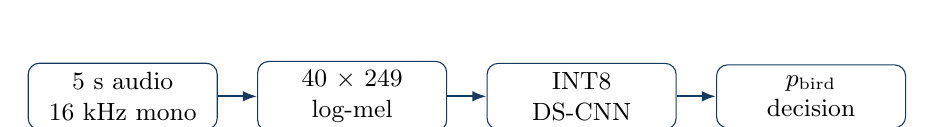
\begin{tikzpicture}[node distance=5mm,box/.style={draw=navy,rounded corners,fill=white,align=center,minimum height=8mm,minimum width=24mm,font=\small},arr/.style={-{Latex[length=1.8mm]},thick,draw=navy}]
\node[box] (a) {5 s audio\\16 kHz mono};
\node[box,right=of a] (b) {40 $\times$ 249\\log-mel};
\node[box,right=of b] (c) {INT8\\DS-CNN};
\node[box,right=of c] (d) {$p_{\mathrm{bird}}$\\decision};
\draw[arr] (a)--(b);\draw[arr] (b)--(c);\draw[arr] (c)--(d);
\end{tikzpicture}
\end{center}
Environmental sensors, LoRaWAN, cloud communication, scheduling, and final battery sizing are intentionally outside the present scope. They are deferred until physical live-audio inference is demonstrated.
\end{summarybox}

\begin{summarybox}{lightgreen}{What has been completed}
\begin{itemize}
  \item Audited the 27-class FSC22 SWinT-BiLSTM Teacher and recovered the correct bird-output mapping: \texttt{birdchirping $\rightarrow$ 12}, \texttt{wingflapping $\rightarrow$ 20}.
  \item Generated deterministic binary Teacher probabilities and trained compact Student models using hard labels plus knowledge distillation.
  \item Performed a KD-weight sweep and selected \textbf{0.8 hard focal loss + 0.2 soft-BCE KD}.
  \item Trained the selected Student on the full dataset and exported FP32 and full-integer INT8 TFLite models.
  \item Reimplemented the full log-mel front-end in C++, verified Python/C++ numerical parity, and replaced the direct DFT with a memory-safe ESP-DSP FFT path.
  \item Added the embedded model asset, TensorFlow Lite Micro wrapper, direct-input smoke test, preprocessing-to-inference firmware, and optimized ESP32S3 build configuration.
  \item All relevant ESP32S3 projects currently \textbf{compile and link successfully}.
\end{itemize}
\end{summarybox}

\boxhead{Selected model and deployment contract}
\begin{center}
\begin{minipage}[t]{0.48\linewidth}
\begin{tabularx}{\linewidth}{>{\bfseries}p{0.43\linewidth}X}
Input duration & 5.0 s \\
Sample rate & 16,000 Hz \\
Samples & 80,000 mono \\
Feature tensor & $40\times249\times1$ \\
Architecture & DS-CNN \\
\end{tabularx}
\end{minipage}\hfill
\begin{minipage}[t]{0.48\linewidth}
\begin{tabularx}{\linewidth}{>{\bfseries}p{0.47\linewidth}X}
Parameters & 32,097 \\
Normalization & $\mu=-9.19348$, $\sigma=3.78920$ \\
Decision threshold & 0.6734629869 \\
INT8 model size & 59,760 bytes \\
Preprocess scratch & 5,124 bytes \\
\end{tabularx}
\end{minipage}
\end{center}

\vspace{3pt}
\boxhead{Model-selection evidence (cross-validation)}
\begin{center}
\begin{tabular}{lrrrrrr}
\toprule
Precision & Recall & F1 & PR-AUC & ROC-AUC & Recall @ FPR=0.02 \\
\midrule
0.728 & 0.873 & 0.780 & 0.905 & 0.986 & 0.860 \\
\bottomrule
\end{tabular}
\end{center}
\textit{Interpretation:} these cross-validation results are the valid model-selection evidence. Metrics obtained after final training on the complete dataset are apparent training metrics and are not presented as independent test performance.

\newpage

{\Large\bfseries\color{navy} Embedded validation status and exact next step}\par
\vspace{3pt}

\begin{summarybox}{lightgreen}{Verified engineering results}
\begin{tabularx}{\linewidth}{X>{\raggedleft\arraybackslash}p{0.21\linewidth}}
Teacher mapping and deterministic soft labels & \verified \\
Student baselines, KD sweep, and selected configuration & \verified \\
FP32/INT8 TFLite export and Keras agreement & \verified \\
Initial Python/C++ preprocessing parity: 99.9598\% exact, max error 1 INT8 unit & \verified \\
Optimized FFT parity: 100\% exact, mean INT8 difference 0 & \verified \\
Memory-safe frame-by-frame preprocessing with ESP-DSP & \verified \\
TFLite Micro wrapper and ESP32S3 compile/link tests & \verified \\
\end{tabularx}
\end{summarybox}

\begin{summarybox}{lightorange}{What has not yet been demonstrated}
\begin{tabularx}{\linewidth}{X>{\raggedleft\arraybackslash}p{0.21\linewidth}}
Five-second waveform capture on the physical board & \pending \\
Physical end-to-end inference on live audio & \pending \\
Measured preprocessing and inference latency & \pending \\
Measured SRAM/PSRAM peaks and runtime stability & \pending \\
Controlled bird/non-bird playback evaluation & \pending \\
Measured energy per classification and final battery capacity & \pending \\
\end{tabularx}
\end{summarybox}

\begin{summarybox}{lightorange}{Current blocker}
The available \textbf{Grove Sound Sensor v1.7} is an analog sound-intensity detector. The manufacturer explicitly states that it should not be used as a recording device. It can later be used as a sound/no-sound trigger, but it cannot provide the five-second waveform required by the classifier.

The prepared live-audio firmware targets the digital PDM microphone on the \textbf{XIAO ESP32S3 Sense expansion board} using:
\begin{center}
\texttt{PDM DATA = GPIO41 \qquad PDM CLK = GPIO42}
\end{center}
That microphone board is not currently available; therefore, physical live-audio validation is blocked by hardware rather than by the trained model or embedded software.
\end{summarybox}

\boxhead{Required purchase}

\textbf{Preferred:} purchase a \textbf{Seeed Studio XIAO ESP32S3 Sense kit} and confirm that it includes the Sense expansion board with the digital microphone. This path matches the PDM firmware already prepared.

\textbf{Alternative:} purchase a digital I2S microphone breakout such as INMP441, ICS-43434, or SPH0645. This is technically valid but requires a new standard-I2S capture backend and explicit wiring.

\begin{summarybox}{lightblue}{Exact next validation after the microphone arrives}
\begin{enumerate}
  \item Capture exactly 80,000 signed 16-bit samples at 16 kHz.
  \item Verify duration, sample count, RMS, peak, DC offset, zeros, and clipping.
  \item Execute the optimized ESP-DSP log-mel preprocessing.
  \item Run the INT8 TFLite Micro Student and report $p_{\mathrm{bird}}$ and the decision.
  \item Record preprocessing latency, inference latency, total latency, internal RAM, and PSRAM.
  \item Test controlled bird and non-bird playback, then measure current during capture, preprocessing, inference, and sleep.
\end{enumerate}
\end{summarybox}

\textbf{Decision requested from supervisor:} approve procurement of the waveform-capable digital microphone hardware and continuation with the physical five-second end-to-end validation. No work on environmental sensors or LoRaWAN is required before this milestone passes.

\vfill
{\footnotesize
\textbf{Repository checkpoint:} \texttt{2f3921e} -- project status and hardware blocker documented.\\
\textbf{Supporting documentation:} full technical report, final Student model card, preprocessing parity reports, and ESP32S3 firmware projects are available in the GitHub repository.\\
\textbf{Hardware references:} \url{https://wiki.seeedstudio.com/xiao_esp32s3_sense_mic/}; \url{https://wiki.seeedstudio.com/Grove-Sound_Sensor/}
}

\end{document}
